\documentclass[10pt]{article}
\usepackage[margin=0.8in]{geometry}
\usepackage[T1]{fontenc}
\usepackage{lmodern}
\usepackage{microtype}
\usepackage{graphicx}
\usepackage{booktabs}
\usepackage{placeins}
\usepackage{xcolor}
\usepackage{hyperref}
\definecolor{navy}{HTML}{16324F}
\definecolor{teal}{HTML}{087E8B}
\hypersetup{colorlinks=true,linkcolor=navy,urlcolor=teal}
\title{\textcolor{navy}{Matched-Opportunity Adaptation}\\[3pt]\large Global and Cluster-Local Refitting Under a Shared Row Budget}
\author{23I-2581 and 23I-2604\\Data Analysis and Visualization --- Phase 3 addendum}
\date{17 November 2026}
\begin{document}\maketitle
\begin{abstract}
This controlled extension holds update clocks and released feedback rows fixed while comparing a frozen classifier with global and cluster-local logistic refits. Thirty paired seeds, three label delays and stationary or abrupt conditional-reversal streams are evaluated. Each adaptive policy receives four opportunities and may use at most 2,000 released rows per opportunity; repeated uses count toward an 8,000-row adaptation cap. Initial training is reported separately.
\end{abstract}
\section{Protocol}
Each stream has 96 batches of 500 rows. The logistic model, scaler and three-cluster MiniBatchKMeans partition are initialized from the 4,000-row training partition; the clusterer is frozen thereafter. Both adaptive policies receive the same latest released row IDs at forecast clocks 25, 49, 73 and 89. The global policy fits one logistic model on the shared window. The local policy fits one replacement model per cluster on that cluster's rows from the same window; a cluster with fewer than 20 rows or a single observed class retains the original global fallback. Its actual fit-row use can therefore be lower than the shared window allowance.

For delay $d$, source batch $s$ can affect forecast batch $b$ only if $s+d<b$. Current-batch labels are excluded before prediction. A fitted label may recur in later windows, and each recurrence counts against the row-use total. Uncertainty resamples paired seeds; batches are not treated as independent replicates.
\section{Results}
\begin{figure}[ht]
\centering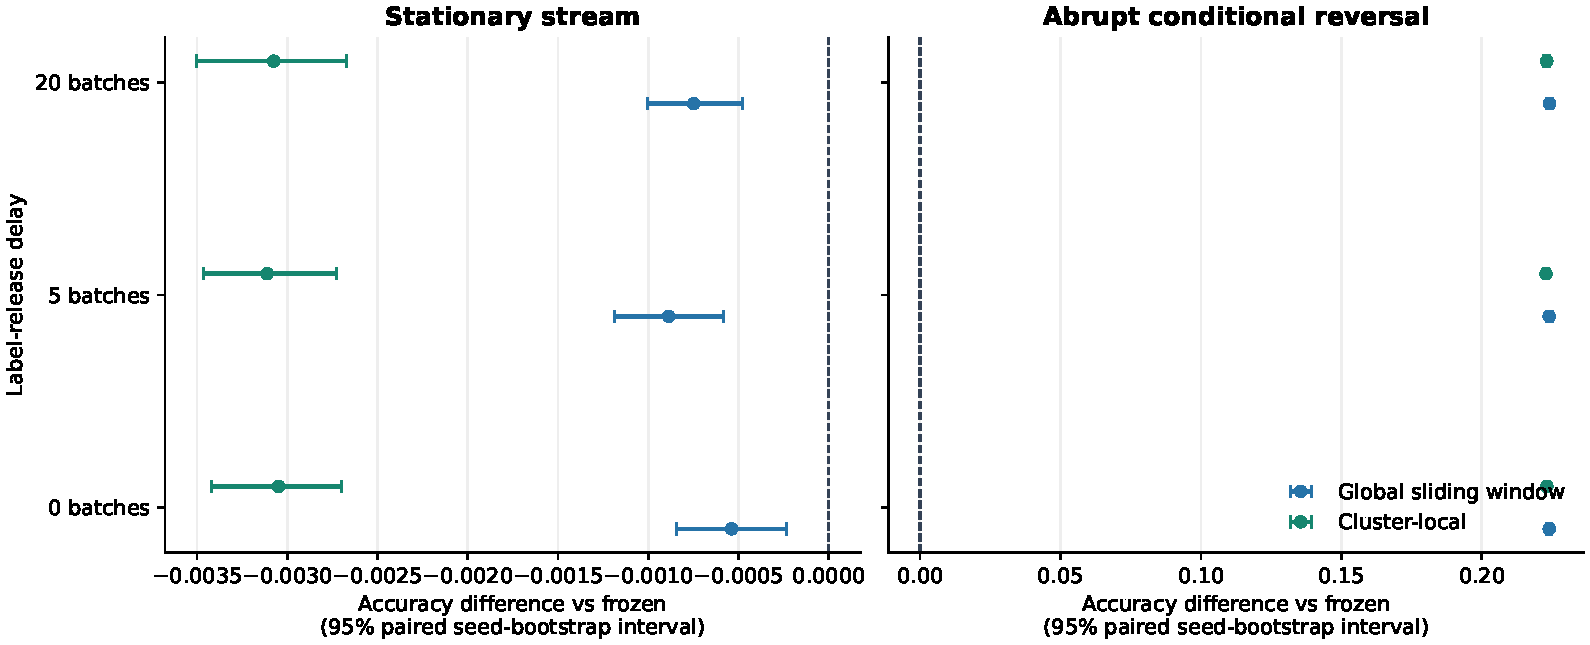
\includegraphics[width=\linewidth]{matched_adaptation_effects.pdf}
\caption{Paired all-stream accuracy differences from the frozen classifier. Each interval is a 95\% bootstrap interval over the 30 matched seeds.}
\end{figure}
\begin{table}[ht]
\centering\small
\begin{tabular}{@{}llrrrrr@{}}
\toprule
Stream & Delay & Frozen & Global & Local & Global rows & Local rows\\
\midrule
Stationary & 0 & 0.724 & 0.724 & 0.721 & 8000 & 8000 \\
Stationary & 5 & 0.724 & 0.724 & 0.721 & 8000 & 8000 \\
Stationary & 20 & 0.724 & 0.724 & 0.721 & 8000 & 8000 \\
Reversal & 0 & 0.388 & 0.612 & 0.611 & 8000 & 8000 \\
Reversal & 5 & 0.388 & 0.612 & 0.611 & 8000 & 8000 \\
Reversal & 20 & 0.388 & 0.612 & 0.611 & 8000 & 8000 \\
\bottomrule
\end{tabular}
\caption{Mean all-stream accuracy and mean cumulative adaptation-row uses per seed. Initial training is excluded from adaptation-row uses.}
\end{table}
For abrupt conditional reversal, local-minus-frozen accuracy differences at delays 0, 5 and 20 are +22.32 pp (+22.23, +22.41); +22.29 pp (+22.18, +22.39); +22.31 pp (+22.21, +22.42) percentage points, respectively; parentheses give 95\% paired seed-bootstrap intervals in percentage points. The estimates describe this fixed generator, partition, window and update schedule. They do not establish superiority on other mechanisms or natural streams.

The matched design answers whether global and local training choices behave differently when their four update opportunities and feedback row windows are held constant. It does not answer whether an error-triggered policy is better than periodic adaptation; that distinct budget-cap comparison is reported in the companion trigger audit. In the stationary condition, updates can be unnecessary by construction, and any accuracy loss is a measured cost rather than a false alarm.

\FloatBarrier
\section{Limitations}
The experiment uses one linear-probabilistic generator, one classifier and one training-fitted three-cluster partition. The local arm sees the same released IDs but fits separate models on region slices; its cumulative model-fit rows are at most the global arm's because disjoint regions partition the shared window. This is not a comparison of equal compute or equal wall time. The row-use cap measures examples passed to fitting, not CPU, memory, energy or acquisition cost. More delays, nonlinear and regional tasks, alternative cluster counts and natural streams remain untested here.

\section{Reproduction}
From the workspace root, run:
\begin{verbatim}
python scripts/run_matched_adaptation_schedule.py
python scripts/report_matched_adaptation_schedule.py \\
  --run results/phase3/matched_adaptation_schedule_20261117_v1 \\
  --out reports/phase3/matched_adaptation_schedule_20261117_v1
tectonic -X compile \\
  reports/phase3/matched_adaptation_schedule_20261117_v1/matched_adaptation_schedule.tex \\
  --outdir reports/phase3/matched_adaptation_schedule_20261117_v1
\end{verbatim}
The run receipt records source, configuration and output hashes; the fit audit stores the shared feedback-ID hash at each update opportunity.
\end{document}
